% MA6223 CA3 report. Build:  tectonic main.tex   (or pdflatex + bibtex, or Overleaf)
% Every number comes from data/ in this repo (see the commands in README.md); nothing is
% typed from memory. Names and the video link live in meta.tex.
\documentclass[conference]{IEEEtran}
\usepackage{amsmath,amssymb,graphicx,booktabs,multirow,xcolor,url}
\usepackage[hidelinks]{hyperref}
\usepackage{iftex}\ifPDFTeX\else\usepackage{fontspec}      % Times under XeTeX (Tectonic); pdflatex needs nothing
\setmainfont{texgyretermes}[Extension=.otf,UprightFont=*-regular,BoldFont=*-bold,ItalicFont=*-italic,BoldItalicFont=*-bolditalic]\fi
\graphicspath{{../figures/paper/}{../figures/}{../v1/paper/figs/}}
\newcommand{\qd}{\dot{q}}
\newcommand{\Js}{{J^{*}}}
% Edit this file only: author names, matric numbers/emails and the OneDrive video link.
% The video must be on an NTU OneDrive with sharing "People in NTU" (Accessible to all NTU).
\newcommand{\videourl}{https://entuedu-my.sharepoint.com/REPLACE-WITH-ONEDRIVE-LINK}
\newcommand{\authorblock}{%
\IEEEauthorblockN{P1 Name\IEEEauthorrefmark{1},
Harshith Gosula\IEEEauthorrefmark{2},
Suhas Suren\IEEEauthorrefmark{3},
P4 Name\IEEEauthorrefmark{4},
P5 Name\IEEEauthorrefmark{5},
Honglin (Alin) Wang\IEEEauthorrefmark{6}}
\IEEEauthorblockA{MA6223 CA3, MSc Robotics and Intelligent Systems, Nanyang Technological University, Singapore\\
\IEEEauthorrefmark{1}Simulation \& integration,
\IEEEauthorrefmark{2}Dynamics,
\IEEEauthorrefmark{3}Control,
\IEEEauthorrefmark{4}Safety,
\IEEEauthorrefmark{5}Experiment \& report,
\IEEEauthorrefmark{6}Arm model}}

\begin{document}

\title{Reactionless Compliance: A Human-in-the-Loop Benchmark of Redundancy Resolution and Contact-Safety
Limits for Teleoperated Free-Floating Space Manipulators}
\author{\authorblock}
\maketitle

\begin{abstract}
A redundant arm on a free-floating servicer turns its own spacecraft whenever it moves, and a 7-joint arm
doing a full 6-D task cannot keep the base still: six task rows and three reactionless rows exceed seven
joints. We built a teleoperation benchmark to measure this trade-off: a momentum-conserving MuJoCo model of
a Kinova Gen3 arm on three servicers (arm-to-base mass ratio 0.30, 0.043, 0.0043), five
redundancy-resolution schemes in 3-D and 6-D variants, a PlayStation~4 interface with haptic warnings, and a
counterbalanced study protocol. On a scripted two-loop orbital-replacement-unit (ORU) task, the reactionless
schemes cut peak base drift by 2.4--2.8$\times$ (3-D) and 1.3--1.4$\times$ (6-D) on the 150\,kg servicer, at the cost of
8--22\,mm of hand error. On the 20\,kg servicer every scheme that finishes the task breaks the
$\pm$5$^\circ$ antenna limit (23--25$^\circ$ in 6-D), and the schemes that respect it cannot finish. For contact safety,
where ISO 10218-1 excludes space robots, we apply the ISO/TS~15066 body model. Simulated impacts show that
the back-drivable joints, not the spacecraft mass, set the effective mass at contact. A pose-dependent
speed limiter built on this keeps all 397 simulated impacts below the ISO force limit (worst 90\,\%).
Human-subject sessions had not been run when this report was written.
\end{abstract}

\noindent\textbf{Video presentation:} \url{\videourl}

\section{Introduction}
On-orbit servicing puts a human operator in charge of an arm whose base is not bolted down. Momentum is
conserved, so every hand motion rotates the servicer and moves its antenna off the ground
station~\cite{dubowsky1993,umetani1989}. A redundant arm can spend its spare joints on cancelling that
reaction~\cite{nenchev1999rns,yoshida2001}. But a 7-joint arm doing a 6-D task (position and orientation)
has one spare joint, and holding the base still needs three. Exact reactionless motion is then impossible,
so every controller trades task accuracy, base drift and posture drift against one another.

Each of the relevant laws exists on paper: damped least squares, gradient projection, null-space impedance,
reaction null-space (RNS) control and impedance inside the RNS~\cite{abiko2006,nakanishi2006}. They have not
been compared under human teleoperation, nor across servicer sizes. Contact safety for such an arm is
also unregulated: ISO~10218-1:2025 excludes space robots~\cite{iso10218}.

\textbf{Contributions.} (i) An open benchmark: three servicers sharing one Kinova Gen3 arm, five schemes in
3-D and 6-D, a scripted closed-loop ORU task, per-tick logging, a fixed tuning rule and a $\beta$-sweep that
traces the 6-D trade-off. (ii) A characterisation of that trade-off and of where base drift breaks a
$\pm$5$^\circ$ pointing limit as the arm-to-base mass ratio changes. (iii) A contact-velocity limit
from the ISO/TS~15066 body model~\cite{iso15066}, calibrated and validated by simulated impacts, and enforced
at run time. (iv) A teleoperation interface (PS4 gamepad, haptics, head-up display) and a
counterbalanced study protocol with an analysis pipeline that runs end to end. Scheme~5 is a known
combination~\cite{abiko2006,nenchev1999impact}; we use it as one condition, not as a claim of novelty.

\section{Related Work}
\textbf{Free-floating kinematics.} The generalized Jacobian~\cite{umetani1989} maps joint rates to hand
motion with the base free; dynamic singularities and the loss of reach follow from it~\cite{dubowsky1993}.
\textbf{Reactionless control.} The reaction null space~\cite{nenchev1999rns,nenchev1999impact} gives joint
motions that leave base attitude unchanged; it was flight-tested on ETS-VII~\cite{yoshida2001}. Bias-momentum
strategies distribute momentum to protect attitude~\cite{dimitrov2004}, and impedance control has been
formulated for free-floating arms~\cite{abiko2006,nakanishi2006}.
\textbf{Redundancy resolution.} The fixed-base classics are gradient projection on a null-space
objective~\cite{liegeois1977} such as manipulability~\cite{yoshikawa1985}, damped least
squares~\cite{wampler1986,deo1995}, weighted least norm for joint limits~\cite{chan1993}, and null-space
impedance~\cite{hogan1985}.
\textbf{Human factors and safety.} Virtual fixtures guide an operator's commands~\cite{rosenberg1993};
predictable motion matters for trust~\cite{dragan2013}; workload is measured with NASA-TLX~\cite{hart1988}.
ISO/TS~15066 gives body-region force limits and a two-body energy model for collaborative robots. To our
knowledge, no prior work compares these schemes with humans in the loop on a free-floating base, or derives a
contact-speed limit for such a base.

\section{System}
\subsection{Servicers and arm}
All three servicers carry the same arm and differ only in the base (Fig.~\ref{fig:lineup},
Table~\ref{tab:servicers}). The arm uses the Kinova Gen3 7-DoF geometry and masses (902\,mm reach,
6.49\,kg moving; MuJoCo Menagerie~\cite{menagerie2022,kinova2020}): roll--pitch--roll--pitch--roll--pitch--roll
joints, pitch limits $\pm$128.9/147.8/120.3$^\circ$ and roll joints limited to $\pm$170$^\circ$.
The joints are velocity servos ($k_v=20$, $\pm$1\,rad/s, torque saturating at $\pm$5\,Nm). The base is a
free body with gravity off. Collisions are on, both arm--base and arm--arm. Simulation uses
MuJoCo~\cite{todorov2012} with RK4 at 0.25\,ms. Control runs at 100\,Hz and holds each command over 40
physics steps.

\begin{figure}[t]\centering
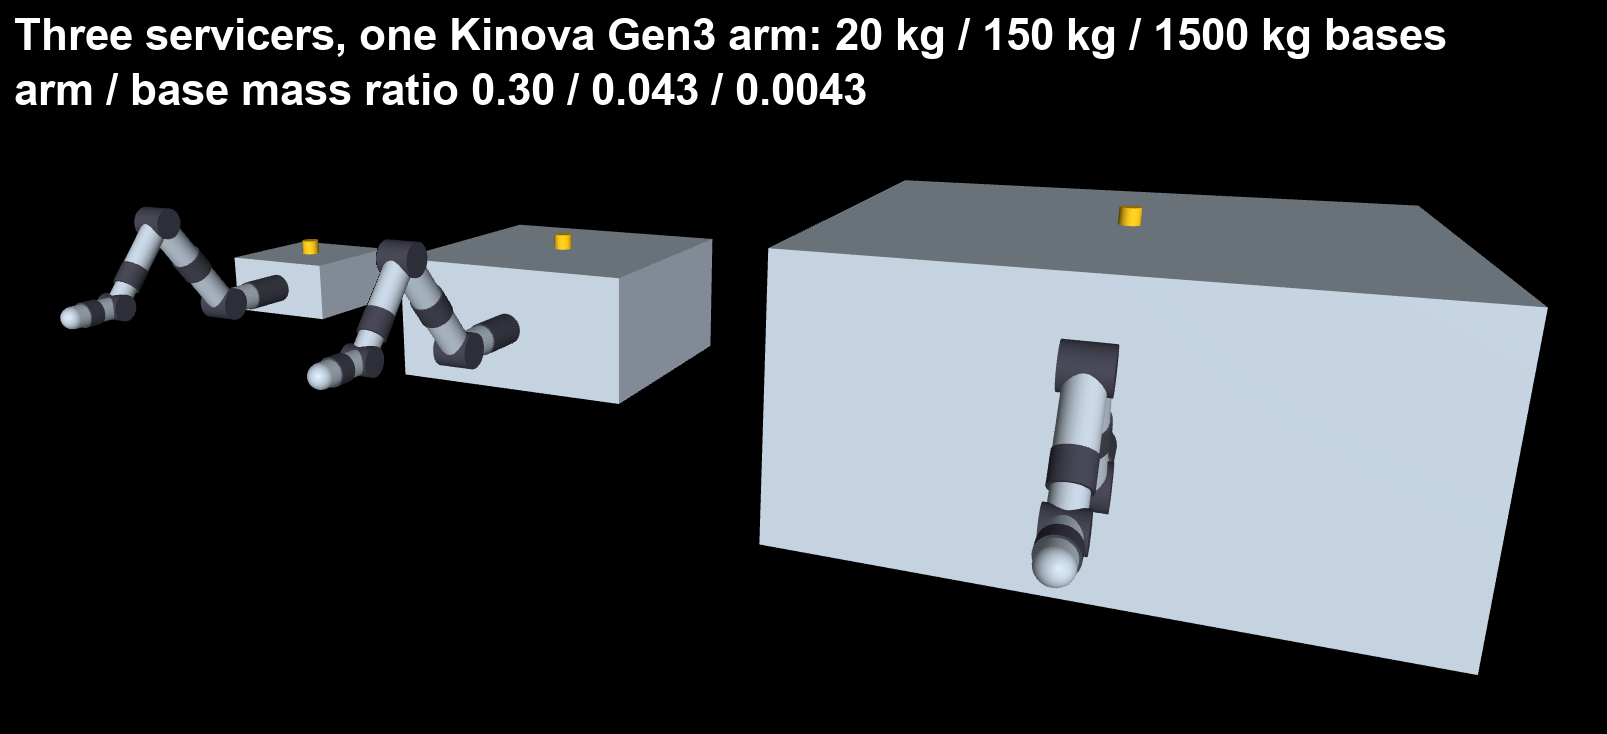
\includegraphics[width=\columnwidth]{render_lineup}
\caption{The three servicers (20, 150, 1500\,kg bases) with the same Kinova Gen3 arm, rendered from the
simulation. The yellow cylinder is the antenna; its boresight must stay within $\pm$5$^\circ$.}
\label{fig:lineup}\end{figure}

\begin{table}[t]\caption{Servicers and the effective mass at the hand (home pose, tool axis)}
\label{tab:servicers}\centering\footnotesize\setlength{\tabcolsep}{4pt}
\begin{tabular}{lccc}\toprule
 & small & medium & large\\\midrule
Servicer mass [kg] & 21.7 & 151.7 & 1501.7\\
Arm / servicer mass ratio & 0.30 & 0.043 & 0.0043\\
$m_{\text{eff}}$, rigid joints [kg] & 27.5 & 149.6 & 1473\\
$m_{\text{eff}}$, limp joints [kg] & 2.56 & 2.56 & 2.56\\
$m_{\text{design}}$ (Sec.~\ref{sec:safety}) [kg] & 8.9 & 11.3 & 37.4\\
$v_{\max}$ design, free/clamped [m/s] & .38/.17 & .34/.15 & .21/.08\\
$v_{\max}$ rigid joints, clamped [m/s] & 0.097 & 0.042 & 0.013\\\bottomrule
\end{tabular}\end{table}

\subsection{Dynamics}
With base twist $v_b$, joint rates $\qd$ and zero initial momentum,
\begin{equation}
H_b v_b + H_{bm}\qd = 0\ \Rightarrow\ v_b = V\qd,\quad V = -H_b^{-1}H_{bm},
\end{equation}
\begin{equation}
\dot x = J_b v_b + J_m\qd = (J_m + J_b V)\qd = \Js\qd .
\end{equation}
$W$, the three angular rows of $V$, maps joint rates to base angular rate. The base attitude is unchanged
exactly when $W\qd = 0$, which uses $W$ rather than the angular rows of $H_{bm}$, because the base frame is
not at the system centre of mass. The momentum gate drives random $\qd$ for 10\,s on every servicer and
checks $\|H_b v_b + H_{bm}\qd\|$ at every physics step. The worst value is $6\times10^{-8}$ against a limit of
$10^{-6}$, and $\Js\qd$ and $W\qd$ match the simulated hand and base velocities to $10^{-7}$. The degree-of-freedom
argument holds numerically at 50 random poses: $[\Js;W]$ has rank 7 of 9 rows in 6-D and rank 6 of 6 in 3-D.

\subsection{Five schemes}\label{sec:schemes}
All schemes output $\qd$ from the operator twist $\dot x_c$. They share a pose servo onto the commanded
target, $\dot x = \dot x_c + K_x e$ ($K_x = 2$\,s$^{-1}$, $e$ clipped at 5\,cm / 0.3\,rad), and one joint
geofence: a joint within 3$^\circ$ of a limit that is still pushing outward is locked and the rest re-solve.
\begin{enumerate}
\item \textbf{DLS:} $\qd = \Js^{\!\top}(\Js\Js^{\!\top}+\lambda^2 I)^{-1}\dot x$~\cite{wampler1986}.
\item \textbf{Gradient projection:} $\qd = \Js^{+}\dot x + (I-\Js^{+}\Js)\,k_g\nabla w(q)$, with $w$ the
manipulability of $\Js$~\cite{liegeois1977,yoshikawa1985}.
\item \textbf{Impedance:} the same null-space form with $\qd_0 = -K_p(q-q_{\text{rest}}) - K_d\qd$~\cite{hogan1985}.
\item \textbf{RNS:} in 3-D, solve $[\Js_{p}; W]\qd = [\dot x_p; -k_a\phi]$ exactly, where $\phi$ is the base
attitude error; in 6-D, see (\ref{eq:wls}) with $\qd_0 = 0$.
\item \textbf{Impedance+RNS:} as 4, with $\qd_0$ injected only through the remaining freedom.
\end{enumerate}
In 6-D, 6 task rows plus 3 reactionless rows exceed 7 joints, so schemes 4 and 5 become a weighted
least-squares problem whose trade-off is set by $\beta$:
\begin{equation}\label{eq:wls}
\min_{\qd}\ \|\Js\qd-\dot x\|^2 + \beta\,\|W\qd + k_{a6}\phi\|^2 + \gamma\,\|\qd-\qd_0\|^2 .
\end{equation}
\textbf{Tuning (no strawmen).} Each scheme's own gain was swept over four values on the medium servicer,
2 loops, in both modes (40 runs). The selection rule was fixed before the runs: among values that finish both
modes, take the lowest summed rms hand error, breaking ties within 10\,\% by peak base drift. Result:
$\lambda=0.01$ (DLS is insensitive between 0.005 and 0.05), $k_g=1$, $K_p=2$ (Impedance), $k_a=1$ (RNS),
$K_p=1$ (Imp.+RNS). The 6-D weights $\beta=3$, $k_{a6}=1$ and $\gamma=10^{-3}$ are the most reactionless
setting with which both schemes 4 and 5 still finish the task on the medium servicer.

\subsection{Teleoperation interface}
Fig.~\ref{fig:hud} shows the operator view: one OpenGL window into which MuJoCo renders. The blue sphere is
the commanded target. The green and yellow lines are the antenna boresight at the start and now, and the
yellow line turns red past 5$^\circ$. The head-up display shows the antenna error, the joint nearest its
limit, arm contact, and the hand speed against the contact limit.
A DualShock~4 is read through SDL2 in a game-style layout: the left stick moves the target relative to the
camera, R2/L2 move it up and down, the right stick orbits the camera, holding R1 switches the stick to
rotation, and holding L1 gives fine control. A southpaw and a world-axis layout are also available.
Haptics use both rumble motors: the heavy motor scales with arm contact force (0.35 at first touch, full at
10\,N), the light motor ramps over the last 15$^\circ$ before a joint limit, and a 250\,ms pulse fires when the
antenna leaves its cone. The scripted task never triggers either motor, so a buzz always means something is
wrong. The mapping was checked on a real controller, and missing input reads as a zero command.

\begin{figure}[t]\centering
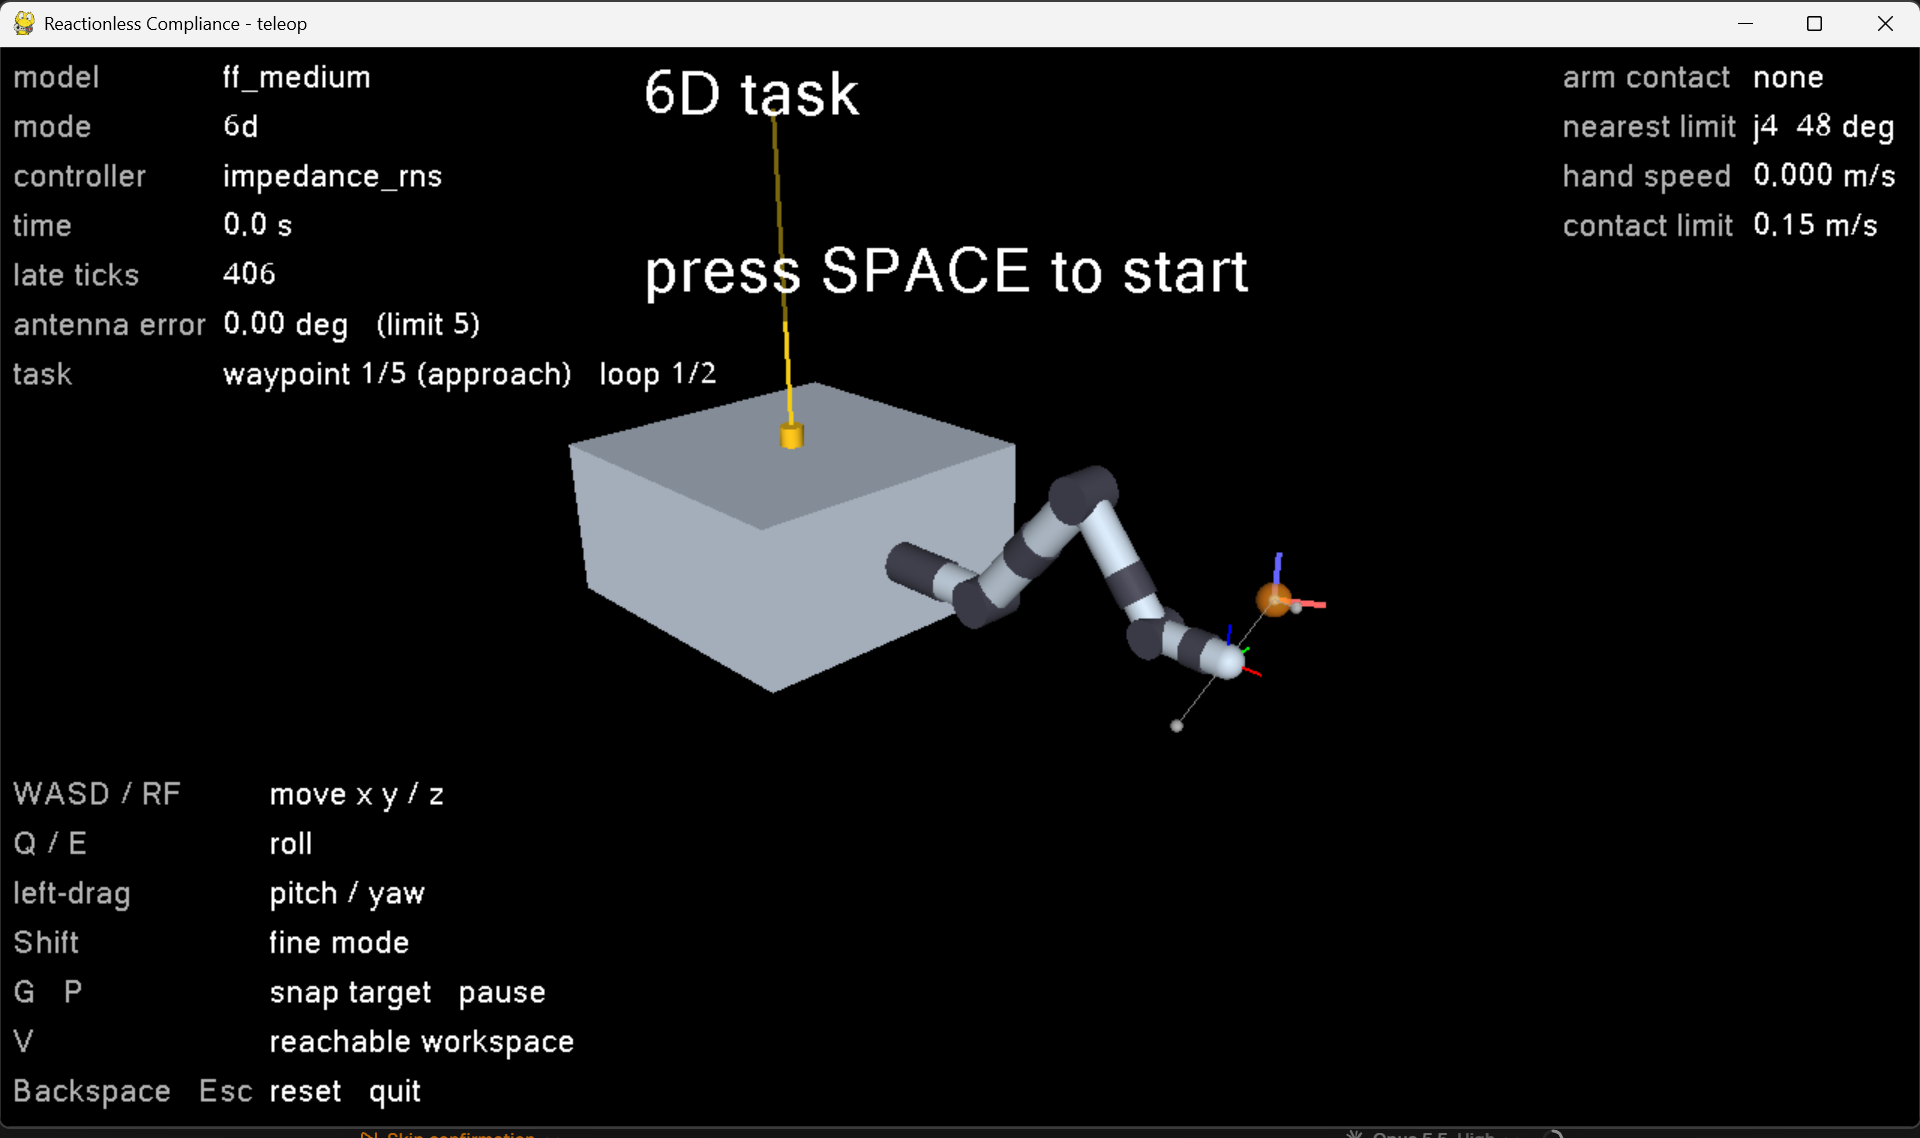
\includegraphics[width=\columnwidth]{screenshot_teleop}
\caption{Participant view at the start of a 6-D trial (medium servicer). Orange: current waypoint with its
target orientation; grey: the ORU loop. Top right: haptic channels and the live contact-speed limit.}
\label{fig:hud}\end{figure}

\subsection{Task}
The task is a closed loop from the hand's home pose, run twice per trial:
start, approach, ORU, approach, stow and back to start, with offsets of up to $\pm$15\,cm and
30$^\circ$. Waypoints are fixed in the world, because the ORU sits on another spacecraft. A waypoint counts
when the real hand stays within 2\,cm (and 10$^\circ$ in 6-D) for 0.3\,s. Returning to the start is what makes
base drift and joint drift $\|q_f-q_0\|$ measurable. Scripted runs follow a minimum-jerk reference at
full-stick speed through the same control loop, logger and safety layer that participants use.

\section{Contact Safety}\label{sec:safety}
\textbf{Body model.} For an arm with effective mass $m_{\text{eff}}(q,u)=1/(u^\top\Lambda_v^{-1}u)$ along
contact direction $u$, the ISO/TS~15066 energy model gives $v_{\max} = F/\sqrt{\mu k}$, with the region's force
limit $F$, spring constant $k$ and effective mass $m_H$ from Annex~A. We include every region that allows
transient contact. Head and face allow none and are handled procedurally (H3). For \emph{free} contact, where
the person can recoil, $F$ is twice the quasi-static limit and $\mu$ is the reduced mass of $m_{\text{eff}}$
and $m_H$. For \emph{clamped} contact, e.g.\ an EVA astronaut in a foot restraint, $F$ is the quasi-static
limit and $\mu=m_{\text{eff}}$. The design case is the worst region and restraint, which is the clamped hand.

\textbf{Which mass hits?} With the joints rigid, the whole spacecraft stands behind the hand: 1473\,kg
on the large servicer, giving a limit of 13\,mm/s (Table~\ref{tab:servicers}). We placed an ISO tissue
spring, backed by $m_H$ (free) or the world (clamped), in front of the hand. We then drove the real servos
into it at 432 random poses and directions: 3 servicers $\times$ 3 body cases $\times$ 0 or 5\,kg payload
$\times$ 24. Pushed across the arm, the $\pm$5\,Nm servos give way, and the peak force hardly depends on
the base mass. The design mass is therefore the limp-joint value plus a calibrated servo share, plus a
small rigid share for pushes along the arm, where the joints have no lever arm:
\begin{equation}
m_{\text{design}} = m_{\text{eff}}^{\text{limp}} + 6\,\text{kg} + 0.02\,m_{\text{eff}}^{\text{rigid}}\cos^2\theta_{u,\text{arm}} .
\end{equation}
\textbf{Limiter and validation.} At run time the commanded $\qd$ is scaled so that the predicted hand speed
$\|\Js\qd\|$ stays below $0.85\,v_{\max}$ along its own direction. To validate this, every impact was
re-run at exactly the limiter's speed and its peak force compared with the ISO limit. All 397 contacts that
occurred stayed below it: worst 0.90 of the limit (clamped hand, push along the arm), median 0.32
(Fig.~\ref{fig:safety}, right; Fig.~\ref{fig:vmax}). We first converted force into an equivalent mass and extrapolated, but that
flagged slow contacts near singularities whose real forces were only 17--33\,N. The direct check is the
honest test. A Monte Carlo sweep of 2700 samples (pose $\times$ direction $\times$ payload 0/2.5/5\,kg
$\times$ restraint $\times$ size) shows why the limiter is needed. At full joint speed, the arm exceeds the
clamped limit in 95--100\,\% of poses. The teleop's own speed cap (0.15\,m/s) exceeds it in every pose
once a 5\,kg payload is attached.

\begin{figure*}[t]\centering
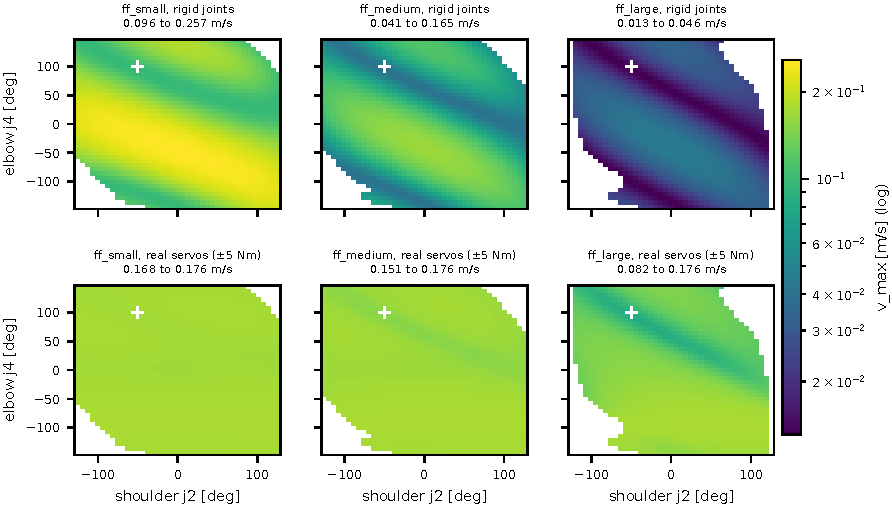
\includegraphics[width=0.82\textwidth]{fig5_vmax}
\caption{Contact-speed limit over shoulder and elbow angle for contact along the tool axis (worst ISO region
and restraint; white: arm inside the base; +: home). Top: rigid joints, which vary 2.7--4.0$\times$ with pose
and fall with servicer mass. Bottom: the real $\pm$5\,Nm servos, nearly flat on the small and medium servicers.}
\label{fig:vmax}\end{figure*}

\begin{figure*}[t]\centering
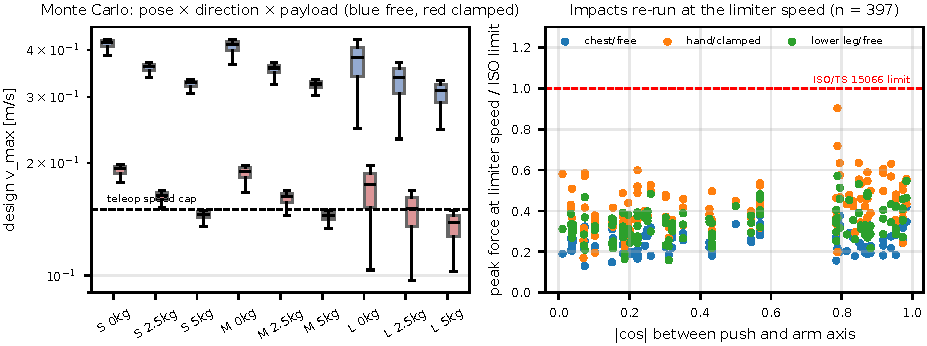
\includegraphics[width=\textwidth]{figS1_safety}
\caption{Left: Monte Carlo design limits (blue free, red clamped contact) per servicer and payload, against the
teleop speed cap. Right: each simulated impact re-run at the limiter speed; every peak force is below its
ISO/TS~15066 limit (worst 0.90).}
\label{fig:safety}\end{figure*}

\section{Experimental Method}
\textbf{Scripted benchmark.} The Week-7 gate runs 5 schemes $\times$ 2 modes $\times$ 3 servicers on the
2-loop task, with a timeout of 1.5$\times$ the reference duration. The $\beta$-sweep runs schemes 4 and 5 in 6-D
at $\beta \in \{0.1,\dots,100\}$ on all servicers (51 runs). Every tick is logged: commands, full state, hand
and target pose, antenna error, haptic channels, limiter scale and camera. Metrics are computed from the
logs, so scripted and human trials share one pipeline.

\textbf{Human-in-the-loop protocol.} The design is within-subject, with 5 schemes $\times$ 2 task modes on
the medium servicer and 2 loops per trial. Modes run as blocks, with odd participants starting in 3-D.
Scheme order within a block follows a Williams Latin square~\cite{williams1949}, and the scheme is hidden
from the participant. The plan is 10--12 participants and $\approx$30\,min per session. After each trial,
participants rate predictability (1--7) and complete raw NASA-TLX~\cite{hart1988}. Analysis uses a Friedman
test with Kendall's $W$, then pairwise Wilcoxon signed-rank tests with Holm correction and effect size $r$.
Below 8 participants, per-participant paired plots replace the inferential tests. One pad layout and the
haptics setting are fixed for all participants. The session runner, questionnaire template, statistics and
figures were all tested end to end on scripted and synthetic data. \emph{At the time of writing no
participant session had been run, so no human results are reported.}

\section{Results}
\subsection{Gate and the cost of reactionless motion}
Table~\ref{tab:gate} and Fig.~\ref{fig:sizes} summarise the gate. All 30 runs were stable, and 26 finished.
Medium and large finished 10/10 each; the four failures are schemes 4--5 on the small servicer.
In 3-D on the medium servicer, RNS and Imp.+RNS cut peak drift from 1.28$^\circ$ (DLS) to 0.53$^\circ$ and
0.46$^\circ$. They finish with 0.059$^\circ$ and 0.001$^\circ$ of base error left. The price is hand error:
13 and 22\,mm rms against 0.6\,mm. Exact reactionless motion is not ``zero drift by construction'' here,
because the $\pm$15\,cm loop leaves the arm's reactionless reach. On the earlier generic arm, raising the weight of the
reactionless rows cut drift to 0.05$^\circ$, but the hand then no longer reached the waypoints.

\begin{table}[t]\caption{Scripted gate, 2 loops (peak / final antenna error in degrees, rms hand error in mm)}
\label{tab:gate}\centering\small\setlength{\tabcolsep}{3pt}
\begin{tabular}{lccccc}\toprule
 & \multicolumn{2}{c}{medium 3-D} & \multicolumn{2}{c}{medium 6-D} & small 6-D\\
Scheme & peak/final & rms & peak/final & rms & peak (done)\\\midrule
1 DLS & 1.28/.040 & 0.6 & 2.03/.407 & 0.6 & 25.3 (yes)\\
2 Grad. proj. & 1.34/.602 & 0.7 & 2.04/.411 & 0.6 & 25.0 (yes)\\
3 Impedance & 1.28/.033 & 0.6 & 1.76/.230 & 0.6 & 22.9 (yes)\\
4 RNS & 0.53/.059 & 13.1 & 1.55/.160 & 8.0 & 1.42 (no)\\
5 Imp.+RNS & 0.46/.001 & 22.5 & 1.44/.154 & 8.7 & 1.45 (no)\\\bottomrule
\end{tabular}\end{table}

\begin{figure*}[t]\centering
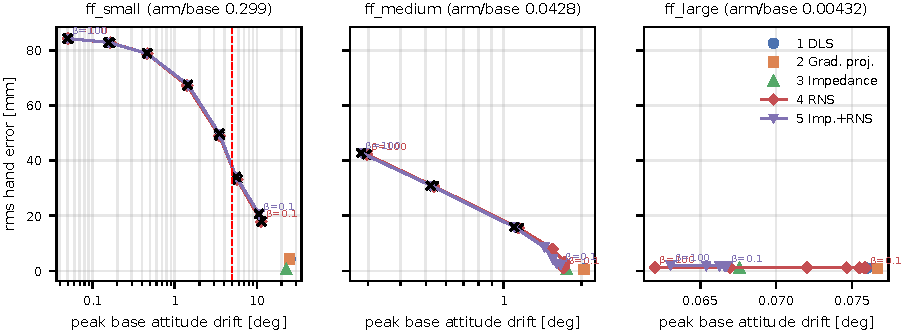
\includegraphics[width=\textwidth]{fig1_tradeoff}
\caption{6-D trade-off from the $\beta$-sweep (curves, schemes 4 and 5) and the single points of schemes
1--3. Black $\times$: task not finished within 1.5$\times$ the reference time. Red dashed line: $\pm$5$^\circ$
antenna limit.}
\label{fig:tradeoff}\end{figure*}

\subsection{The 6-D trade-off}
Fig.~\ref{fig:tradeoff} plots hand error against peak base drift. On the medium servicer, raising $\beta$
from 0.1 to 100 moves Imp.+RNS from 2.3\,mm and 1.66$^\circ$ to 42.8\,mm and 0.28$^\circ$. The task is still
completed up to $\beta=3$; beyond that the hand misses the 2\,cm tolerance. Schemes 1--3 sit at the
accurate end (0.6\,mm, 1.76--2.04$^\circ$). On the large servicer the trade-off vanishes: every scheme stays
under 0.08$^\circ$ with about 1--2\,mm of error, so the choice of scheme does not matter there.

\begin{figure*}[t]\centering
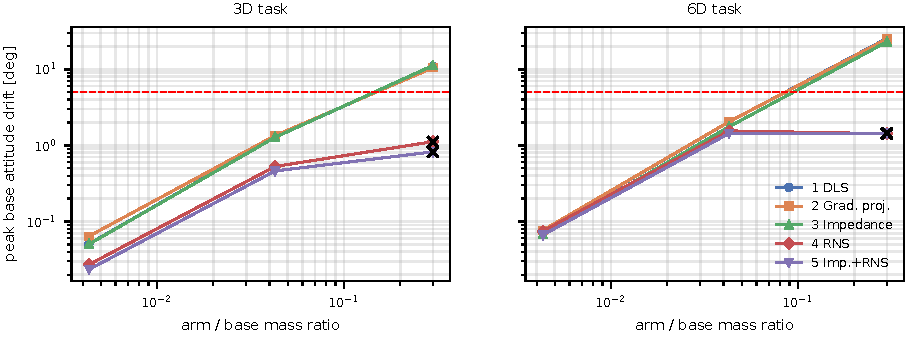
\includegraphics[width=0.9\textwidth]{fig2_size}
\caption{Peak base drift against arm-to-base mass ratio for the 3-D and 6-D tasks ($\times$: task not finished;
red: $\pm$5$^\circ$ antenna limit).}
\label{fig:sizes}\end{figure*}

\begin{figure*}[t]\centering
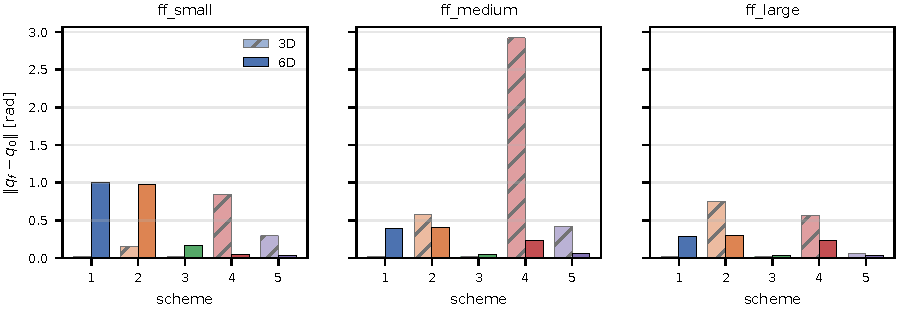
\includegraphics[width=0.9\textwidth]{fig3_joint_return}
\caption{Joint-configuration return error $\|q_f-q_0\|$ after two loops (hatched 3-D, solid 6-D), per scheme and servicer.}
\label{fig:joints}\end{figure*}

\subsection{When does drift matter?}
Drift scales roughly with the mass ratio (Fig.~\ref{fig:sizes}). Fig.~\ref{fig:demo} shows the small-servicer case in the demo video. On the 20\,kg servicer (ratio
0.30) the schemes split into two groups. Schemes 1--3 finish but peak at 22.9--25.3$^\circ$ in 6-D and
10.4--11.2$^\circ$ in 3-D, which loses the radio link. Schemes 4--5 stay under 1.5$^\circ$ but cannot reach the
waypoints. In the $\beta$-sweep, holding the base within 5$^\circ$ needs $\beta\ge 1$, and no $\beta$ then
finishes the task. For this arm, a CubeSat-class servicer cannot do the task within the pointing limit with
any of the five schemes. The 150\,kg servicer can, and the 1500\,kg servicer does not need reactionless
control at all.

\begin{figure}[t]\centering
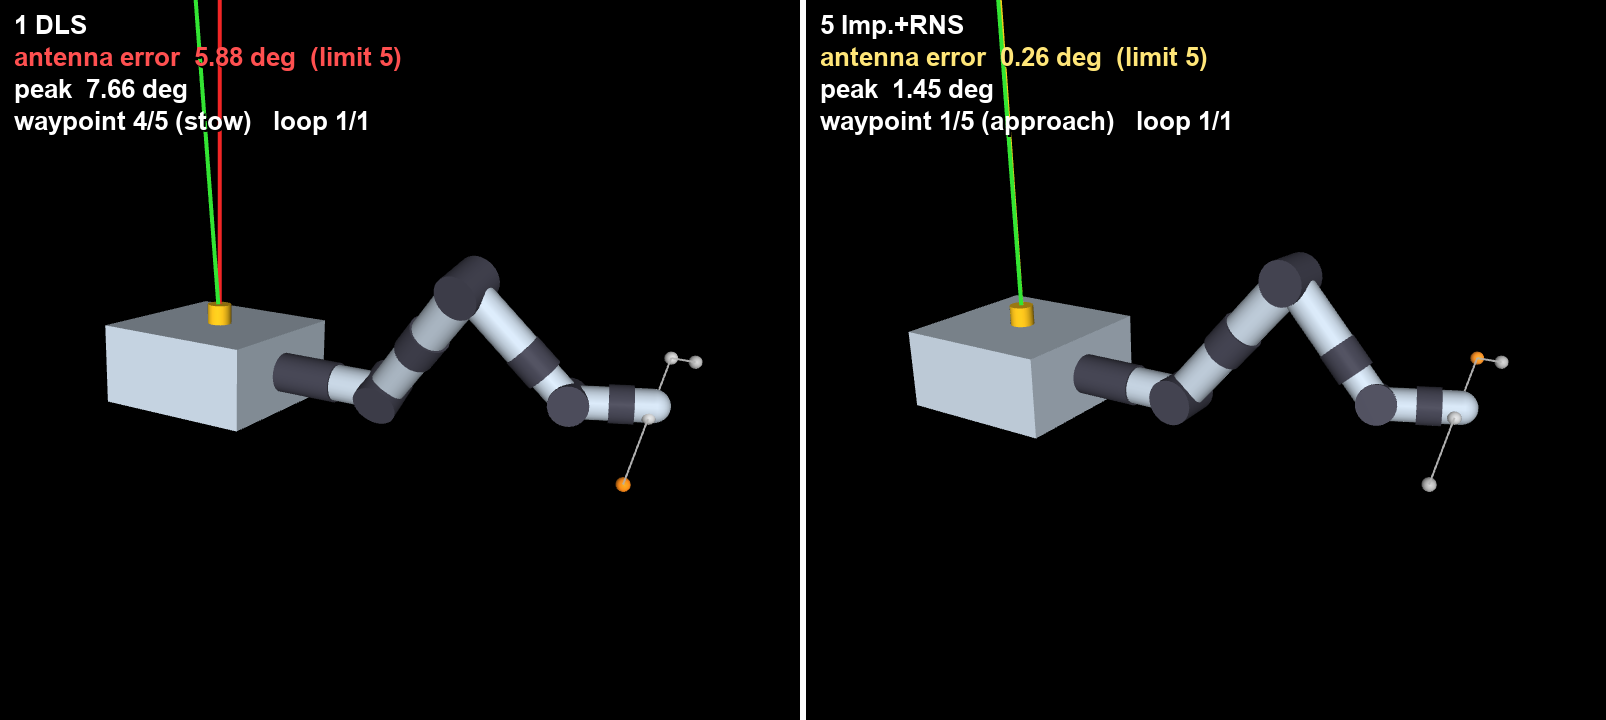
\includegraphics[width=\columnwidth]{demo_frame}
\caption{Frame from the demo video: the same scripted 6-D operator input on the 20\,kg servicer. DLS (left)
follows the loop but tips the antenna past 5$^\circ$ (red line; peak 19$^\circ$ in the one-loop clip); Imp.+RNS
(right) holds 0.26$^\circ$ but is still at the first waypoint.}
\label{fig:demo}\end{figure}

\subsection{Posture drift}
Returning the hand does not return the arm (Fig.~\ref{fig:joints}). Without a posture term, joint drift is
large: RNS ends 2.92\,rad away in 3-D on medium and gradient projection 0.58\,rad. With posture
impedance, Impedance ends 0.016\,rad away and Imp.+RNS 0.065\,rad (6-D). The plain RNS drift also explains
its one verification failure (R4 below). Its joints wander through the null space, and the base finishes
0.059$^\circ$ off, while Imp.+RNS finishes 0.001$^\circ$ off. Posture impedance is what makes reactionless
control repeatable for an operator.

\subsection{Safety case}
The verification matrix is generated from the data (\texttt{docs/SAFETY.md}). It covers ten hazards, including
antenna loss, an astronaut strike, a head strike, self-collision, joint limits, singularities, a wrong
dynamics model, operator confusion, input loss and an infeasible 6-D demand. Table~\ref{tab:verify} lists
the requirements. The limiter acted in at most 3.9\,\% of ticks, all on the large servicer during
along-arm motion, and the worst hand speed reached 0.84 of $v_{\max}$.

\begin{table}[t]\caption{Verification matrix (computed from data)}\label{tab:verify}
\centering\small\setlength{\tabcolsep}{3pt}
\begin{tabular}{p{0.07\columnwidth}p{0.47\columnwidth}p{0.38\columnwidth}}\toprule
Req & Requirement & Result\\\midrule
R1 & Antenna within $\pm$5$^\circ$, 2 loops, 6-D & Pass on medium and large; fail on small\\
R2 & Contact speed $\le v_{\max}(q)$ & Pass: 397/397 impacts under the limit\\
R3 & Momentum residual $<10^{-6}$ & Pass ($6\times10^{-8}$)\\
R4 & 3-D reactionless: final $<0.05^\circ$, peak $\le\frac12$ DLS & \textbf{Fail}: RNS medium 0.059$^\circ$\\
R5 & No joint past its limit & Pass (min.\ margin 2.4$^\circ$)\\
R6 & No bus contact in task; contact signalled & Pass\\
R7 & $|\qd|\le1$\,rad/s, direction kept & Pass\\
R8 & 6-D reactionless infeasible, 3-D exact & Pass (rank 7/9, 6/6)\\
R9 & No head or face contact & Open (procedural)\\
R10 & Missing input $\Rightarrow$ zero command & Pass (CI)\\\bottomrule
\end{tabular}\end{table}

\subsection{Operator aid: the tilt-limit map}
In parallel work on an earlier, generic 12.5\,kg arm model (repository \texttt{v1/}), P2 asked a different
question: can the operator \emph{see} which targets the base can afford before commanding them?
Probing 98 directions from rest gives three nested cages for 0.5, 1 and 2$^\circ$ of base tilt
(Fig.~\ref{fig:opview}). On 300 targets near the edge, the 2$^\circ$ cage was right on 271, with 8 false
``go'' and 21 false ``no-go''. A runtime fence held the base at most 2.02$^\circ$ on 46 commands that a
rehearsal had refused. The cost of such a wrong command was time (median 11--14\,s), not attitude. The
limit binds only in a band of spacecraft sizes, about 150--600\,kg at 2$^\circ$. This agrees with the
benchmark result that drift matters on the small and medium servicers and not on the large one.

\begin{figure}[t]\centering
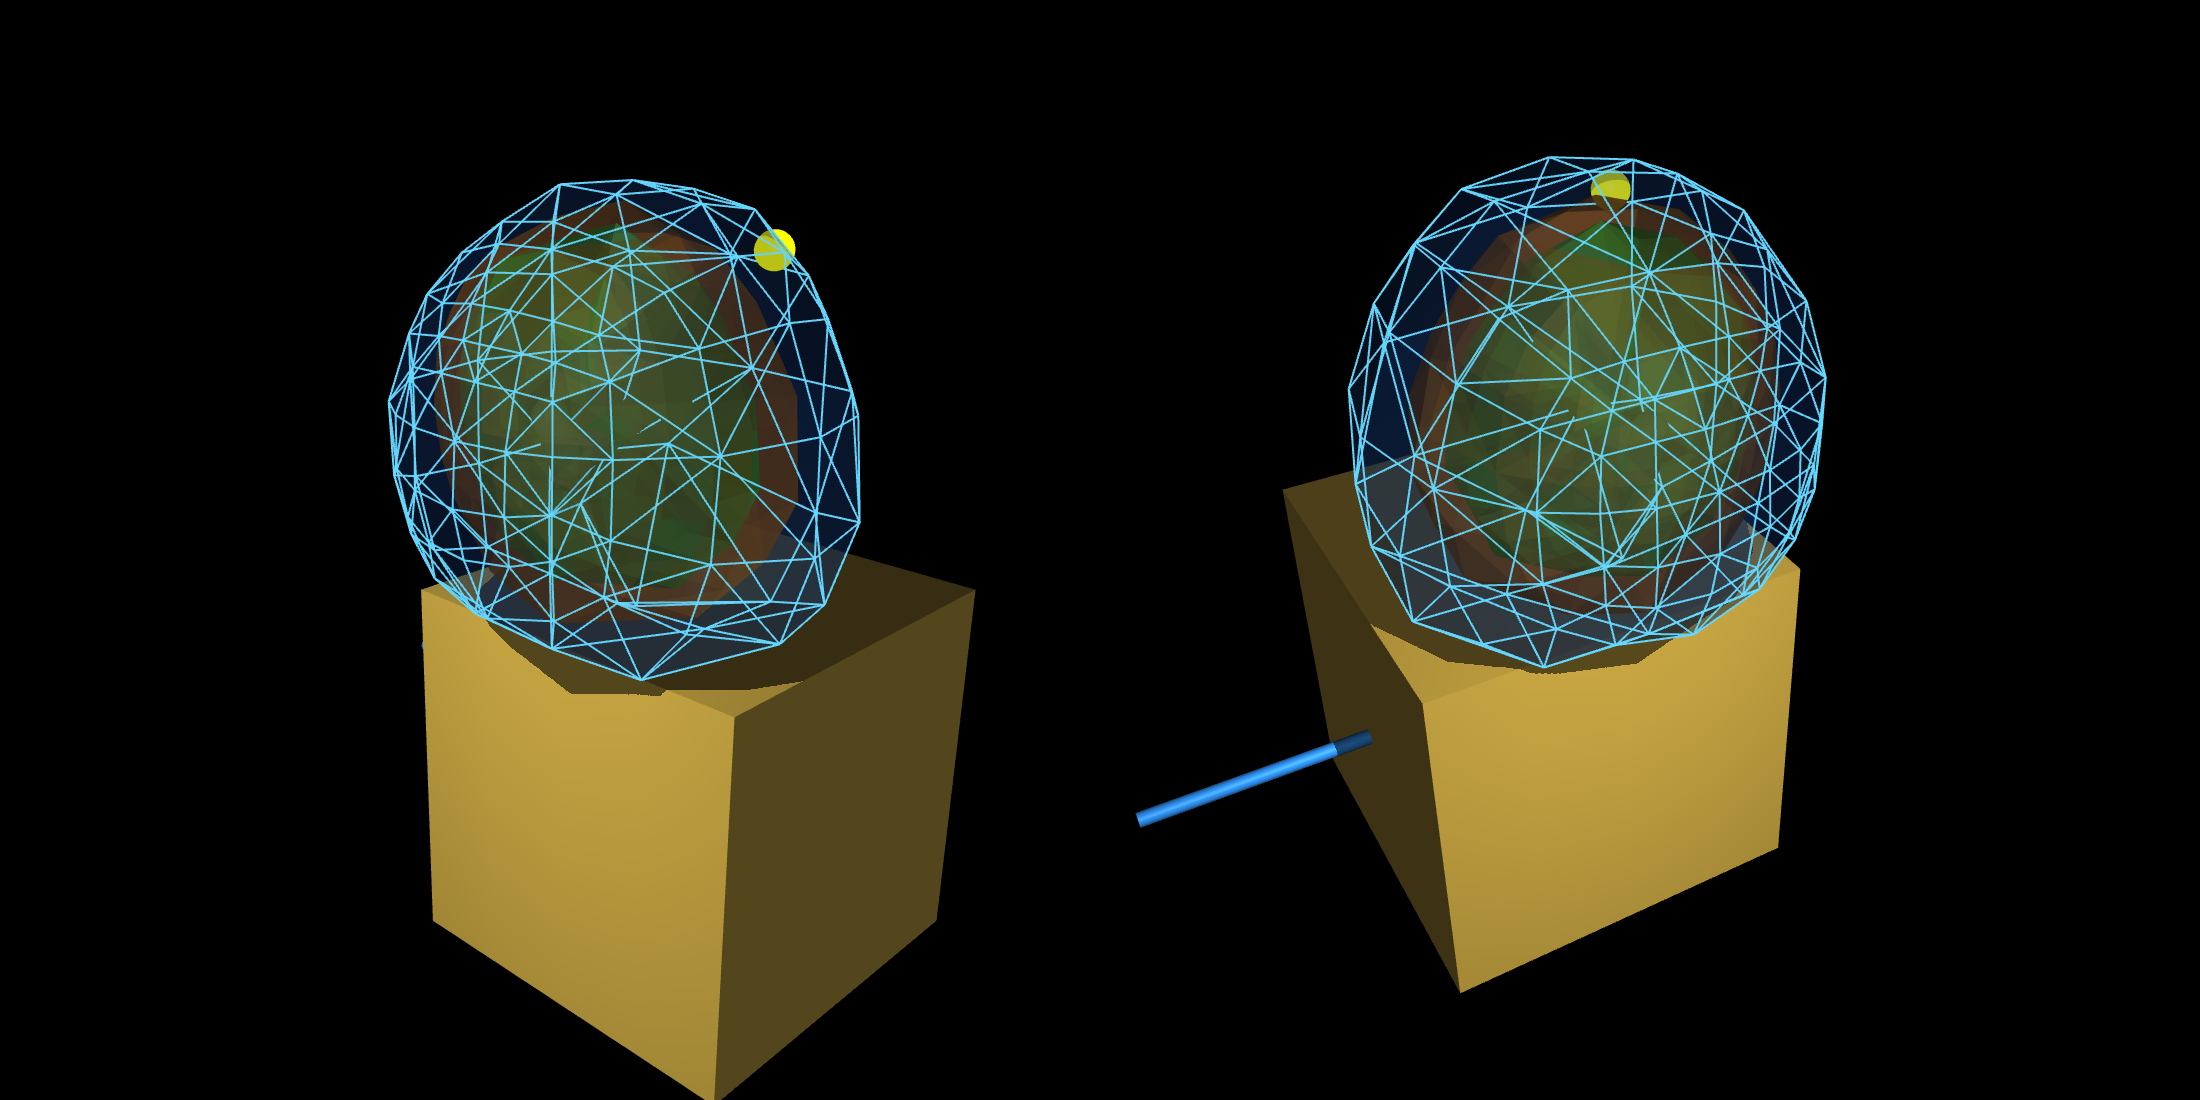
\includegraphics[width=\columnwidth]{fig_opview}
\caption{Tilt-limit cages around the hand (v1 model, 300\,kg): blue, 2$^\circ$; orange, 1$^\circ$; green,
0.5$^\circ$ of base tilt. The yellow target lies in the caution zone.}
\label{fig:opview}\end{figure}

\section{Discussion and Limitations}
\textbf{What the trade-off means for mission design.} The mass ratio decides which scheme is right.
Above about 0.1 no scheme meets a 5$^\circ$ pointing limit for this task, and the operator needs attitude
control or a smaller workspace. Near 0.04 the reactionless schemes buy a 1.3--2.8$\times$ reduction in peak
drift for centimetre-level hand error. Imp.+RNS adds the posture repeatability that plain RNS lacks. Below
0.005 DLS or Impedance is simpler and just as good. Fig.~\ref{fig:tradeoff} lets a mission choose $\beta$
from its pointing budget.

\textbf{Safety.} Joint compliance, not the spacecraft, sets the contact limit. With the real servos,
$v_{\max}$ varies little over the workspace (0.15--0.18\,m/s on medium), whereas rigid joints give 0.04--0.17\,m/s.
The plan's expectation of a strongly pose-dependent limit holds only for rigid joints, such as an arm with
brakes engaged. The clamped case dominates, and a payload of a few kilograms lowers the limit below what
the interface can command, so the limiter is not optional.

\textbf{Limitations.} Everything here is simulated. No participant data exists yet, and the benchmark's
human half is pending. Other limitations:
\begin{itemize}
\item \textbf{Model:} one arm, rigid links, no friction, flexible appendages, sensor noise or initial
momentum; attitude control is off, though real servicers usually keep it on.
\item \textbf{Drives:} the real Gen3 joints give about 39/9\,Nm, not our $\pm$5\,Nm.
\item \textbf{Safety assumptions:} the 6\,kg servo share is calibrated on our servo model and must be
re-measured for real drives. The tissue model is the ISO spring with $e=0$. The v1 tilt-limit map comes
from a different arm model.
\item \textbf{Tuning:} gains were tuned on scripted input, and a human may prefer different ones.
\end{itemize}

\section{Conclusion}
A 7-joint arm on a free-floating servicer cannot track a 6-D task, keep its base still and keep its posture
at once. The benchmark makes the trade-off concrete. On a 150\,kg servicer, reactionless schemes cut drift by
1.3--2.8$\times$ for 8--22\,mm of hand error. On a 20\,kg servicer no scheme both finishes the task and keeps
the antenna within 5$^\circ$. On a 1500\,kg servicer the problem disappears. Posture impedance is what makes
reactionless control repeatable. For contact safety, back-drivable joints shield the person from the
spacecraft's mass. A limiter calibrated by simulated impacts keeps every tested impact within ISO/TS~15066
force limits. The interface, protocol and analysis are ready for the human study.

\bibliographystyle{IEEEtran}
\bibliography{refs}
\end{document}
